\documentclass{article}

    \usepackage[utf8]{inputenc}
    \usepackage[T1]{fontenc}
    \usepackage{aeguill}
    % \usepackage[francais]{babel}
    \usepackage[a4paper]{geometry}
    \usepackage{array}
    \usepackage{amsfonts}
    \usepackage{amsmath} 
    \usepackage{amssymb}
    \usepackage{amsthm}
    \usepackage{xspace}
    \usepackage{dsfont}
    \usepackage{collcell}
    \usepackage{datatool}
    \usepackage{enumitem}
    \usepackage{xstring}
    \usepackage{booktabs}
    \usepackage{environ}
    \usepackage{bbm}
    \usepackage{hyperref}
    \usepackage{graphicx}
    \usepackage{caption}
    \usepackage{stmaryrd}
    \usepackage[dvipsnames]{xcolor}
    \usepackage{tikz}
    \usetikzlibrary{trees}
    \usepackage{ulem}
    \usepackage{cancel}
    \usepackage{pgfplots}
    % \usepackage{minted}
    % \usemintedstyle{monokai}
    \usepackage{multicol}
    
    \pgfplotsset{compat=newest}
    \usetikzlibrary{automata} % LATEX and plain TEX
    \usetikzlibrary[automata] % ConTEXt
    \usetikzlibrary{arrows}
    \usetikzlibrary{automata,arrows,positioning,calc}
    \xdefinecolor{vertf}{named}{OliveGreen}
    \xdefinecolor{rougef}{named}{BrickRed}
    \xdefinecolor{bleuf}{named}{BlueViolet}
    \newcommand{\Var}{vecteur aléatoire réel\xspace}
    \newcommand{\var}{variable aléatoire réelle\xspace}
    \newcommand{\ssi}{si et seulement si\xspace}
    \newcommand{\cad}{c'est-à-dire\xspace}
    \newcommand{\fdr}{fonction de répartition \xspace}
    \newcommand{\pp}{\mathbb P}
    \newcommand{\un}{\mathbbm{1}}
    \newcommand{\esp}{\mathbb E}
    \newcommand{\vari}{\mathbb V}
    \newcommand{\cov}{\text{Cov}} 
    \newcommand{\gras}{\textbf}
    \newcommand{\itemb}{\item[$\bullet$]}
    \newcommand{\rouge}{\textcolor{red}}
    \newcommand{\bleu}{\textcolor{blue}}
    \newcommand{\rougef}{\textcolor{rougef}}
    \newcommand{\vertf}{\textcolor{vertf}}
    \newcommand{\bleuf}{\textcolor{bleuf}}
    \newcommand{\limn}{\underset{n\rightarrow +\infty}{\lim}}
    \newcommand{\flechn}{\underset{n\rightarrow +\infty}{\longrightarrow}}
    \newcommand{\RR}{\mathbb R}
    \newcommand{\Q}{\mathbb Q}
    \newcommand{\N}{\mathbb N}
    \newcommand{\Z}{\mathbb Z}
    \newcommand{\R}{\mathbb R}
    \newcommand{\D}{\mathbb D}
    \newcommand{\C}{\mathbb C}
    \newcommand{\Rn}{\mathbb R^n}
    \newcommand{\Rp}{\mathbb R^p}
    \newcommand{\Rq}{\mathbb R^q}
    \newcommand{\brn}{\mathcal B(\mathbb R^n)}
    \newcommand{\brp}{\mathcal B(\mathbb R^p)}
    \newcommand{\brq}{\mathcal B(\mathbb R^q)}
    \newcommand{\br}{\mathcal B(\mathbb R)}
    \newcommand{\brbarre}{\mathcal B(\overline{\mathbb R}}
    \newcommand{\pps}{P-presque-sûrement\xspace}
    \newcommand{\mespos}{\mathcal M^+(\mathcal B(\mathbb R^n),\mathcal B(\overline{\mathbb R}))}
    \newcommand{\cvps}{\xrightarrow[n\rightarrow\infty]{p.s.}}
    \newcommand{\cvld}{\xrightarrow[n\rightarrow\infty]{L^2}}
    \newcommand{\cvlp}{\xrightarrow[n\rightarrow\infty]{L^p}}
    \newcommand{\cvp}{\xrightarrow[n\rightarrow\infty]{\mathbb P}}
    \newcommand{\cvloi}{\xrightarrow[n\rightarrow\infty]{\mathcal L}}
    \newcommand{\definition}{\vspace{0.5cm}\begin{tcolorbox}[colback=bleuf!5!white,colframe=bleuf!75!black,title=Définition]}
    \newcommand{\propriete}{\vspace{0.5cm}\begin{tcolorbox}[colback=bleuf!5!white,colframe=bleuf!75!black,title=Propriété]}
    \newcommand{\proprietee}{\vspace{0.5cm}\begin{tcolorbox}[colback=red!5!white,colframe=red!75!black,title=Propriété]}
    \newcommand{\theoreme}{\vspace{0.5cm}\begin{tcolorbox}[colback=red!5!white,colframe=red!75!black,title=Théorème]}
    \newcommand{\lemme}{\vspace{0.5cm}\begin{tcolorbox}[colback=red!5!white,colframe=red!75!black,title=Lemme]}
    \newcommand{\proposition}{\vspace{0.5cm}\begin{tcolorbox}[colback=red!5!white,colframe=red!75!black,title=Proposition]}
    \newcommand{\fin}{\end{tcolorbox}\vspace{0.5cm}}
    \newcommand{\preuve}{\noindent\uline{Preuve :}\xspace}
    \newcommand{\remarque}{\noindent\uline{Remarque :}\xspace}
    \newcommand{\exemple}{\noindent\uline{Exemple :}\xspace}
    \newcommand{\rappel}{\noindent\uline{Rappel :}\xspace}
    \newcommand{\notation}{\noindent\uline{Notation :}\xspace}
    
    
    % transposition de tableaux
    
    
    \usepackage{booktabs,array}
    \def\Midrule{\midrule[\heavyrulewidth]}
    \newcount\rowc
    
    \makeatletter
    \def\ttabular{%
    \hbox\bgroup
    \let\\\cr
    \def\rulea{\ifnum\rowc=\@ne \hrule height 1.3pt \fi}
    \def\ruleb{
    \ifnum\rowc=1\hrule height 1.3pt \else
    \ifnum\rowc=6\hrule height \heavyrulewidth 
       \else \hrule height \lightrulewidth\fi\fi}
    \valign\bgroup
    \global\rowc\@ne
    \rulea
    \hbox to 10em{\strut \hfill##\hfill}%
    \ruleb
    &&%
    \global\advance\rowc\@ne
    \hbox to 10em{\strut\hfill##\hfill}%
    \ruleb
    \cr}
    \def\endttabular{%
    \crcr\egroup\egroup}
    
    
    \usepackage{tcolorbox}
    
    

    \hypersetup{colorlinks=true,linkcolor=black}
    
    \usepackage{fancyhdr}
    \pagestyle{fancy}
    \lfoot{S. DO }
    \rfoot{\thepage}
    \cfoot{ }
    \lhead{DEEP LEARNING FOR NAMED ENTITY RECOGNITION}
    \chead{ }
    \rhead{  }
    
    \renewcommand{\footrulewidth}{1pt}
    
    \newcommand{\ind}{\setlength\parindent{0.5cm}} 
    
\begin{document}
    
    \begin{titlepage} 


     \begin{flushright}
     \includegraphics{logo-ensae.jpg}
     \end{flushright}
    \vspace*{\stretch{0.5}}
    \hrulefill
    \begin{center}\Huge
    Deep Learning for Named Entity Recognition \\ 
    \end{center}
    \hrulefill
    \vspace*{1cm}
    \begin{center} \Large
    S. Do
    \end{center}
    \vspace*{\stretch{1}}
 
     \begin{flushright}
         June - October 2018
     \end{flushright}
    \end{titlepage}
    
\newpage


\newpage
\section*{Introduction}


This short document is extracted from the report that I wrote
for a summer internship during my first year of master's 
degree in ENSAE Paristech in 2018. \\ \par 
 It consists of a short
 introduction to basic concepts in Deep Learning 
 applied to Natural Language Processing. It thus aims at 
 recalling Deep Learning basics, introducing word embeddings,
  describing some popular NLP networks as LSTMs, and finally
   describing a 2016 NER architecture using all the
    aforementioned concepts. \\ \par 
    Future versions of this report 
    might include more recent concepts as attention learning, 
    question answering systems, etc. 
\newpage 


\newpage
\tableofcontents
\newpage 



\newpage

\section{Deep Learning Basics}

We begin by first laying the basis of Deep Learning, as it is the starting
point of modern NLP techniques. To do so, we will first introduce 
the neuron concept and modelisation. Then, we will describe 
feed-forward neural networks (FFNNs), and finally we will show how to train
FFNNs using backpropagation. 

\subsection{Neuron}
The idea of copying and simplifying the most important cell in the human 
brain was first explored by Rosenblatt's Perceptron, described in 1957 in \cite{Perceptron}. Some changes 
have been made since this first modelisation, but it stills somewhat 
ressembles the biological model of a neuron : a biological neuron receives
signals from other neurons and outputs a signal in response, depending on some 
activation rules. 
An artificial neuron does approximately the same thing : 
it takes $n$ signal inputs $(x_1, x_2, ..., x_n)$, and outputs the signal $y = f(w_1  x_1 + ... + w_n  x_n)$, 
where $f$ is called the \textit{activation function}, and $w_1, ..., w_n$ are called the weights 
of the neuron. \\

\noindent Basically, if $f = Id$, the neuron performs a linear regression 
of $y$ on the $(x_i)_{i=1, ..., n}$ by fitting the weights on sample data. 

\noindent Usually, chosen activation functions are the sigmoid ($\sigma$), the hyperbolic tangent ($\tanh$) or the ReLU functions:
\begin{eqnarray*}
    \forall x \in \R, \sigma(x) &=& \frac{1}{1+e^{-x}} \\
    \forall x \in \R, \tanh(x) &=& \frac{e^{2x}-1}{e^{2x}+1} \\
    \forall x \in \R, \text{ReLU}(x) &=& \max(0, x) 
\end{eqnarray*}

\vspace{1cm}
\begin{center}
    \captionof{figure}{Most common activation functions plots}
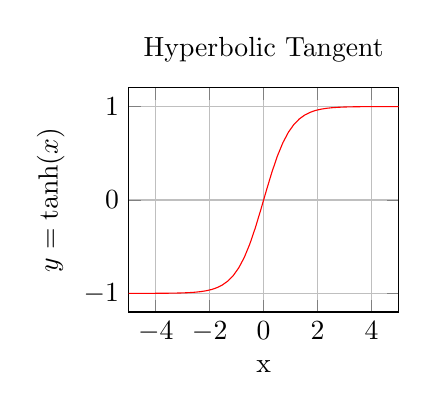
\begin{tikzpicture}
    \begin{axis}[xmax=5,
                 xmin = -5,
                 samples=50,
                 grid=major,
                 xlabel={x },
                 ylabel={$y=\tanh (x)$},
                 title={Hyperbolic Tangent},
                 scale = 0.5]
    \addplot[red]{(e^(2*x)-1)/(e^(2*x)+1)};
    \end{axis}
\end{tikzpicture}
    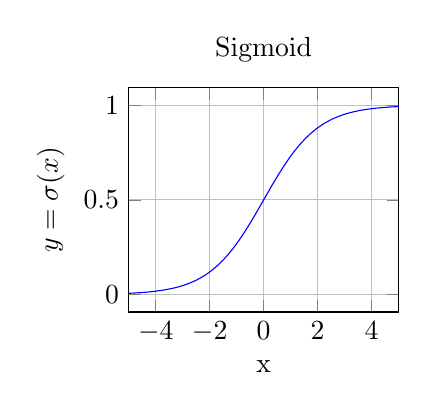
\begin{tikzpicture}
        \begin{axis}[xmax=5,
                     xmin = -5,
                     samples=50,
                     grid=major,
                     xlabel={x},
                     ylabel={$y = \sigma(x)$},
                     title={Sigmoid},
                     scale = 0.5]
        \addplot[blue]{1/(1+e^(-x))};
        \end{axis}
\end{tikzpicture}
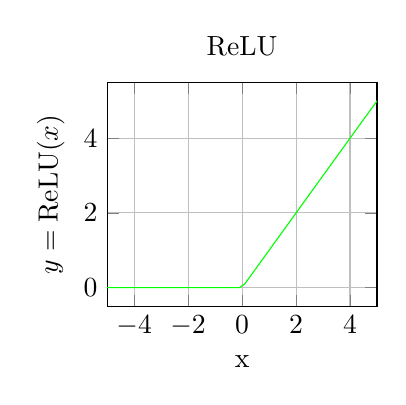
\begin{tikzpicture}
    \begin{axis}[xmax=5,
                 xmin = -5,
                 samples=50,
                 grid=major,
                 xlabel={x},
                 ylabel={$y = \text{ReLU}(x)$},
                 title={ReLU},
                 scale = 0.5]
    \addplot[green]{max(0,x)};
    \end{axis}
\end{tikzpicture}
\end{center}

\noindent Functions such as sigmoid and hyperbolic tangent
are chosen for their non-linear and bounded nature. 
Neurons are usually schematized as in Figure \ref{figure:neuron}.
\newpage
\begin{center}
    \captionof{figure}{Representation of a neuron}
    \label{figure:neuron}
\tikzstyle{inputNode}=[draw,circle,minimum size=10pt,inner sep=0pt]
\tikzstyle{stateTransition}=[->]
\begin{tikzpicture}
	\node[draw, circle, minimum size=25pt, inner sep=0pt] (x) at (0,0) {};

	\node[inputNode] (x0) at (-2, 1.5) {$\tiny x_0$};
	\node[inputNode] (x1) at (-2, 0.75) {$\tiny x_1$};
	\node[inputNode] (x2) at (-2, 0) {$\tiny x_2$};
	% \node[inputNode] (x3) at (-2, -0.75) {$\tiny x_3$};
	\node[inputNode] (xn) at (-2, -1) {$\tiny x_n$};

	\draw[stateTransition] (x0) to node [midway, sloped, above = 0.01] {$w_0$} (x);
	\draw[stateTransition] (x1) to node [midway, sloped, above = 0.01] {$w_1$} (x);
	\draw[stateTransition] (x2) to node [midway, sloped, above = 0.01] {$w_2$} (x);
	% \draw[stateTransition] (x3) to node [midway, sloped, above = 0.01] {$w_3$} (x);
	\draw[stateTransition] (xn) to node [midway, sloped, above = 0.01] {$w_n$} (x);
	\draw[stateTransition] (x) -- (3,0) node [midway,above=0.1cm] {$f(\sum_{i = 1}^n w_i x_i)$};
	% \draw[dashed] (0,-0.43) -- (0,0.43);
	\node (dots) at (-2, -0.35) {$\vdots$};
\end{tikzpicture}
\end{center}

Though, modelling data with a single neuron doesn't bring any innovation : it is like doing linear, 
logistic, or censored regressions. Therefore, neurons are never used alone : the interesting thing with neurons
is to stack them and turn this into a \textit{network}. We thus explain the simplest model of neural network: 
the feed-forward neural network. 

\subsection{Feed-Forward Neural Networks}\label{sec:ffnns}

The feed-forward neural network (FFNN) stacks and parallelizes neurons, as schematized in Figure \ref{figure:ffnn}. 
In a network containing $L\in \N$ hidden layers, size $n_1, n_2, ..., n_L$ respectively,
the inputs of the network are first fed to the first layer's neurons ($n_1$ neurons). Each neuron
has its own weights and computes an output to the signal he receives from the inputs. The $n_1$ generated outputs
are then fed to the $n_2$ neurons of the next layer, and so on. 


\tikzset{%
  every neuron/.style={
    circle,
    draw,
    minimum size=1cm
  },
  neuron missing/.style={
    draw=none, 
    scale=1.5,
    text height=0.333cm,
    execute at begin node=\color{black}$\vdots$
  },
}

\begin{center}
\captionof{figure}{Representation of a feed-forward neural net with a single hidden layer}
\label{figure:ffnn}
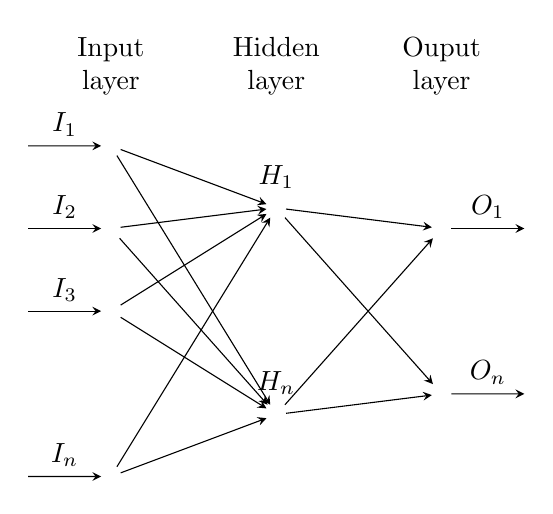
\begin{tikzpicture}[x=1.5cm, y=1.5cm, >=stealth, scale = 0.7]

\foreach \m/\l [count=\y] in {1,2,3,missing,4}
  \node [every neuron/.try, neuron \m/.try] (input-\m) at (0,2.5-\y) {};

\foreach \m [count=\y] in {1,missing,2}
  \node [every neuron/.try, neuron \m/.try ] (hidden-\m) at (2,2-\y*1.25) {};

\foreach \m [count=\y] in {1,missing,2}
  \node [every neuron/.try, neuron \m/.try ] (output-\m) at (4,1.5-\y) {};

\foreach \l [count=\i] in {1,2,3,n}
  \draw [<-] (input-\i) -- ++(-1,0)
    node [above, midway] {$I_\l$};

\foreach \l [count=\i] in {1,n}
  \node [above] at (hidden-\i.north) {$H_\l$};

\foreach \l [count=\i] in {1,n}
  \draw [->] (output-\i) -- ++(1,0)
    node [above, midway] {$O_\l$};

\foreach \i in {1,...,4}
  \foreach \j in {1,...,2}
    \draw [->] (input-\i) -- (hidden-\j);

\foreach \i in {1,...,2}
  \foreach \j in {1,...,2}
    \draw [->] (hidden-\i) -- (output-\j);

\foreach \l [count=\x from 0] in {Input, Hidden, Ouput}
  \node [align=center, above] at (\x*2,2) {\l \\ layer};

\end{tikzpicture}

\end{center}

One important thing about feed-forward neural networks is the word "forward" in their name.
Indeed, FFNNs only pass the information they get forward to the next layer. There isn't any kind
of recurrence in them, and that's what makes FFNN so simple. Their apparent simplicity is though capable
of approximating any measurable function, even with a single hidden layer, if the dimensions of the layer(s) are 
large enough, as proven in Kurt Hornik, 1989 \cite{Hornik1989}. Not all networks keep their "forward"
character : for instance, neural nets such as RNNs and LSTMs introduce recurrence. Their are 
developped in section \ref{subsec:lstm}.\\ \\
For further developments, let's adopt the following notations : let $L$ be the number of hidden 
layers, and $n_l$ the number of neurons in the layer $l$. The $i$-th neuron in the $l$-th layer is
noted $N_i^{(l)}$. \\


\noindent $N_i^{(l)}$ has $n_{l-1}$ weights : let $w_{k, i}^{(l)}$ be the weight of the edge linking 
$N_{k}^{(l-1)}$ to $N_i^{(l)}$.
 If we denote $z_i^{(l)}$ the output of $N_i^{(l)}$, then it can be computed with:

\begin{align*}
    z_i^{(l)} = f \left ( \sum_{k=1}^{n_{l-1}} w_{k, i}^{(l)} z_{k}^{(l-1)} \right )
\end{align*}

\noindent with $f$ the activation function of $N_i^{(l)}$ (to simplify notations, we put the same activation to all
neurons and all layers). \\

\noindent If we now denote $Z^{(l)} = (z_i^{(l)})_{i=1, ..., n}$, we then have the following matrix notation
for layer $l$:
\begin{align*}
    Z^{(l)} = f \left ( W^{(l)} Z^{(l-1)} \right )
\end{align*}
\noindent where $f$ is of course applied to each coordinate of $W^{(l)} Z^{(l-1)}$,
 and with $W^{(l)} \in \R^{n_{l}\times n_{l-1}}  $ : 
\begin{align*}
    W^{(l)} = 
    \left (
    \begin{array}{ccc}
        w_{1, 1}^{(l)} & \hdots & w_{n_{l-1}, 1}^{(l)} \\
        w_{1, 2}^{(l)} & \hdots & w_{n_{l-1}, 2}^{(l)} \\
        \vdots & & \vdots \\
        w_{1, n_l}^{(l)} & \hdots & w_{n_{l-1}, n_l}^{(l)} \\
    \end{array}
    \right )
\end{align*}
The set containing all the weights matrices will be denoted $\mathcal{W} := {W^{(l)}}_{l=1, ...L}$ for further use.\\ \\


A question remains for the output layer. If the aim is to do a regression, then classic 
activation functions are used. However, when trying to do classification, the ouput layer
is a little bit modified. For a problem with $K$ classes, the size of the ouput layer is 
set to $N^{(l)} = K$, and the chosen "activation" function is the softmax function : 
\begin{align*}
    \forall i = 1, ..., K , z_{i}^{(L)} &:= \frac{e^{a_i^{(L)}}}{\sum_{k=1}^{K} e^{a_k^{(L)}}}
\end{align*}
where $\forall i = 1, ..., K, a_i^{(L)} :=  \sum_{k=1}^{n_{l-1}} w_{k, i}^{(l)} z_{k}^{(l-1)}$



\noindent This function represents the probability for an input $x$ to belong to the $i$-th class. \\ \\


The weights, the architecture, and the activation functions thus entirely define the network. Still, 
weights are an unknown parameter that has to be estimated with data. Let's go back to the classic 
statistical learning paradigm and let $(x_i, y_i)_{i=1, ..., n}$ be our independant observations, drawn from an unknown probability distribution function called $P$. 
When a given $x_i$ is fed to the network, weighted sums are computed in all layers, activation
functions are activated, and finally the network outputs a $\hat{y}_i = \text{FFNN}(x_i|\mathcal{W})$ response. 
Our aim is to learn the weights $\mathcal{W}$ from the data by minimizing the error between 
$y_i$ and $\hat{y}_i$. We thus have to define a loss functions, which quantifies this error. 
A standard expression of our minimization problem that sums up all this could be the following: find $\mathcal{W}*$ so that:

\begin{align*}
    \mathcal{W}* \in    \arg \underset{\mathcal{W}}{\min}   \
     \mathcal{L}(\mathcal{W}) + \lambda \Phi(\mathcal{W})
\end{align*}

With $\mathcal{L}$ being the empirical risk term, or the \textbf{loss function}, and $\lambda\Phi$
being a regularization term. 
Regarding regression, usual losses apply : mean squared error (MSE), $\mathcal{L}_2$ loss function, 
mean absolute error, $\mathcal{L}_1$ loss function, etc... Still, some other useful losses are 
used in deep learning, as the Kullback Leibler divergence. Regarding classification, usual loss functions 
are the following : cross-entropy, negative logarithmic likelihood, hinge loss, etc. We recall the expression
of the loss function that is going to be useful for the following : the cross-entropy. \\ \\
Cross-entropy loss is adapted to networks in which the output layer function is a softmax, 
or more generally to a function that returns the probability to belong to each class. This loss
comes from the negative logarithmic likelihood :
\begin{align*}
    \mathcal{L}((x_i, y_i)_{i=1, ..., n}) = -\sum_{i=1}^n \ln p(y_i|x_i, \mathcal{W})
\end{align*}
We need to define more precisely what $p(y_i|x_i, \mathcal{W})$ really is. As we are in a classification
context, we could write the $(y_i)_i$ as one-hot vectors: if a given example $y_i$ belongs to 
the j-th class, then $y_i$ is a vector of zeros excepted on its $j$-th coordinate, which is a one. 
By denoting $C_k$ the $k$-th class, we have:
\begin{align*}
    p(y_i  |x_i, \mathcal{W}) = \prod_{k=1}^K p(C_k|x_i)^{y_{i, k}}
\end{align*}
where $y_{i, k}$ is the $k$-th coordinate of $y_i$ sample. As $p(C_k|x_i)$ is the result $\hat{y}_{i, k}$ of our
softmax function, we can finally re-write :

\begin{align*}
    \mathcal{L}(x_i, y_i) = -\sum_{k=1}^K y_{i,k}\ln (\hat{y}_{i, k})
\end{align*}


\subsection{Backpropagation Algorithm}


\noindent Now that we have chosen a loss function to quantify the estimation error made by the network,
we can write the gradient that we would like to compute in order to minimize the loss over all observations
contained by our dataset:
\begin{align*}
    \frac{\partial \mathcal{L}((x_i, y_i)_{i=1, ..., n})}{\partial \mathcal{W}} = 
    \sum_{i=1}^n \frac{\partial \mathcal{L}(x_i, y_i)}{\partial \mathcal{W}} 
\end{align*}

\noindent Unfortunately, the loss $\mathcal{L}(x_i, y_i)$ is difficult to differentiate with respect to 
$\mathcal{W}$, as  $\mathcal{L}(x_i, y_i) = -\sum_{k=1}^K y_{i,k}\ln (\hat{y}_{i, k})$ and $\hat{y}_{i, k} = z_{i, k}^{(l)}$ 
results from a complex computation regarding the weights of the networks. The \textbf{backpropagation}
algorithm tries to solve this problem by doing the following : 
\begin{itemize}
    \item It starts first by computing, for a given $x$, the output $\hat{y} = \text{FFNN}(x)$. This is called the forward pass. 
    \item Then, we are interested in quantifying the variation of the error when weights from the output layer 
    change. In other words, we are interested in computing:
    \begin{align*}
        \frac{\partial \mathcal{L}(x, y)}
        {\partial w_{i, j}^{(L)}}
    \end{align*}
    Using chain rule, we have:
    \begin{align}
        \frac{\partial \mathcal{L}(x, y)}
        {\partial w_{i, j}^{(L)}} &= \sum_{k=1}^K
        \frac{\partial \mathcal{L}(x, y)}
        {\partial a_k^{(L)}} \
        \frac{\partial a_k^{(L)}}{\partial w_{i, j}^{(L)}} \label{eq:backprop1}\\
        &= 
        \frac{\partial \mathcal{L}(x, y)}
        {\partial a_j^{(L)}} \
        \frac{\partial a_j^{(L)}}{\partial w_{i, j}^{(L)}} \label{eq:backprop2}\\
        &= \delta_j^{(L)} \
          z_i^{(L-1)} \label{eq:backprop3}
    \end{align}
    (\ref{eq:backprop2}) is obtained from the fact that if $k\neq j$, then $ \frac{\partial a_k^{(L)}}{\partial w_{i, j}^{(L)}} = 0$
    and (\ref{eq:backprop3}) is obtained from  the definition of $a_j^{(L)} = \sum_{k=1}^{K} w_{k, j} z_{j}^{(L)}$ which gives: 
    $\frac{\partial a_j^{(L)}}{\partial w_{i, j}^{(L)}} = z_j^{(L-1)}$ 
    Finally, $\delta_j^{(L)}$ is defined as $\delta_j^{(L)} = \frac{\partial \mathcal{L}(x, y)}
    {\partial a_j^{(L)}}$ 
     
    
     \item Let's now interest ourselves in $\delta_j^{(l)}$, for any $l=1, ..., L-1$. Using chain rule, 
     \begin{align}
        \delta_j^{(l)} &= \sum_{k=1}^{n_{l+1}}
        \underset{= \delta_k^{(l+1)}}{
        \underbrace{
        \frac{\partial \mathcal{L}(x, y)}{\partial a_k^{(l+1)}}}} \
        \frac{\partial a_k^{(l+1)}}{\partial a_j^{(l)}}  \label{eq:backprop4}
     \end{align}
     And we also have by definition: 
     \begin{align}
         a_k^{(l+1)} &= \sum_{k'=1}^{n_{l}}  w_{k', k}^{(l+1)} f(a_{k'}^{(l)}) \\
         \Leftrightarrow \frac{\partial a_k^{(l+1)}}{\partial a_j^{(l)}} &= 
         w_{j, k}^{(l+1)} f'(a_j^{(l)})
     \end{align}
     Thus, (\ref{eq:backprop4}) can be re-written as follows:

     \begin{align}
         \delta_j^{(l)} &= f'(a_j^{(l)}) \sum_{k=1}^{n_{l+1}} \delta_k^{(l+1)}  w_{j, k}^{(l+1)} 
        \label{eq:backprop5}
        \end{align}
which defines some kind of inverse recurrence relationship. \newpage
\item Finally, the three following equations resolve our problem :
\[\left \{\begin{array}{cclr}
    \frac{\partial \mathcal{L}(x, y)}{\partial w_{i, j}^{(l)}}
    &= &\delta_j^{(l)} \ z_i^{(l-1)} & \ \ \forall l = 1, ..., L-1\\
    \delta_j^{(l)} 
    &= &f'(a_j^{(l)}) \sum_{k=1}^{n_{l+1}} \delta_k^{(l+1)}  w_{j, k}^{(l+1)} & \ \ \forall l = 1, ..., L-1\\
    \frac{\partial \mathcal{L}(x, y)}{\partial w_{i, j}^{(L)}}
    &= &\delta_j^{(L)} \ z_i^{(L-1)}&
\end{array} \right . \]
Those three equations mean that if we can compute the gradients with respect to the weights 
of the last layer, then, with the second equation of the system, we are able to go a step backward, 
and compute the gradients with respect to the weights of the previous layer. By backward induction, 
all gradients with respect to all weights can be computed. 
\end{itemize}
The backpropagation algorithm is at the heart of deep learning. The process, proposed in 
1986 indepently by the Rumelhart, Hinton and William team and Yann LeCun, gave a new breath 
to neural network theory, allowing to train efficiently FFNNs on more and more powerful computers.
Even in more advanced architectures as LSTMs, the backpropagation algorithm holds with small modifications. \\ \\ 

\noindent Once gradients can be computed thanks to the backpropagation algorithm, 
various optimizers can be used to minimize the loss function. In deep learning, most common 
optimizers are Adam optimizer, or the stochastic gradient descent (SGD). During the learning 
process, the training dataset is divided into batches, passed one by one to the optimizer. 
The dataset is generally seen many times by the network, with different batches division, or with batches presented in 
different order. The process of seeing one time the whole dataset is called an epoch. Training a NN on
100 epochs means seeing 100 times the whole dataset. \\ \\

Now that we know how to train a FFNN, we can introduce a simple, but very effective FFNN that 
learns continuous and dense word representations : the Word2Vec.



















\newpage
\section{Continuous Representation of Words}\label{sec:word2vec}


Representing words as vectors is a difficult task, and the idea has been 
explored since at least the 1970s, when word vector space models were created. 
There are many reasons for representing words as vectors: float vectors are 
a good input to other models, the kind of inputs learning theory
has been designed for. 
For numerous reasons, many simple models provide a sparse and high-dimensionnal 
representation of words : for instance, the simplest model, one-hot encoding, causes sparsity 
and high-dimension as in this model, given a vocabulary $V$ of size 
$|V|$, each word $w\in V$ is represented by a one-hot vector $x_w\in\R^{|V|}$. 


Trying to address this issue in word representation, people have been
searching for dense and continuous representation of words, leading to a 
groundbreaking article by Mikolov and al., 2013 \cite{NIPS2013_5021b},   
\cite{Mikolov2013EfficientSpace}.
 Their approach uses simple feed-forward neural networks. In this section, we will detail 
Mikolov's Word2Vec architecture, and learning techniques. Word2Vec is a generic word for two neural networks architectures, Skip-Gram and 
Continuous Bag-of-Words (CBOW), proposed by Mikolov et al., 2013, \cite{Mikolov2013EfficientSpace}. 
These networks aims both at a \textit{fake task}: predicting the neighbourgh words 
surrounding a given word for Skip-Gram, predicting a word from its context for CBOW. 
In this section, we are going to focus on the Skip-Gram model.  We will first describe the architecture, 
as in the first paper \cite{Mikolov2013EfficientSpace}
, and then we will discuss further methods, described in \cite{NIPS2013_5021b}, 
adopted to learn the representations more efficiently.


\subsection{Skip-Gram Architecture}

The Skip-Gram architecture is the one of a single hidden-layer neural network, as it can be seen in Figure
\ref{fig:skipgram}. Learning pairs proposed to the network are a word ($w_t$) as the input and its context with respect
to a certain window size $C$ : ($w_{t-k}, ..., w_{t-1}, w_{t+1}, ... w_{t+k}$) as the ouput, so as to the network
can learn to predict a context by its center words. In order words, the network performs a classification :
each word being a class, the network tries to link a class to a set of $C$ (the window size) classes
( = the $C$ surrounding words). 
 As the networks performs a classification, 
 the ouput layer's activation function is a softmax.  


\begin{center}
    \captionof{figure}{Representation of skip-gram}
    \label{fig:skipgram}
    \includegraphics[scale=0.35]{skip-arch}
\end{center}

Inputs and outputs are clear, but the projection layer is still a little bit mysterious. It in fact
consists of $N\in \N$ neurons, where $N$ is the size of the embeddings that we want. 
The activation function is the identity for all $N$ neurons. If the vocabulary size is $V\in \N$, 
the number of classes is also $V$ (each unique word is a class). Thus, the dimension of the weight 
matrix $W = W^{(1)}$, linking the inputs to the projection layer, is of size $(V, N)$. \\

We then define for a given one-hot encoded word $X$ its embedding, called $X_{\text{emb}}$ by the following:
\begin{align}
    X_{\text{emb}} = X^{T}  W 
    \label{eq:embeddinform}
\end{align}
\begin{align*}
    X  =
    \left (
    \begin{array}{c}
        0 \\
        \vdots \\
        0 \\
        1 \\
        0 \\
        \vdots \\
        0
    \end{array}
    \right ) \in \{ 0, 1\}^{V}
    , \ \
    W = \left (
    \begin{array}{ccc}
        w_{1,1} & \dots & w_{1, N} \\
        \vdots  &       & \vdots \\
        w_{V,1} & \dots & w_{V, N} \\ 
    \end{array}
    \right ) \in \R^{(V, N)}, \ \ 
    X_{\text{emb}} \in \R^{N}
\end{align*}


The question of the chosen training loss is left for section \ref{subsec:negsamp}, where learning 
process and improvements are described more completely.  \\ 

An important thing to note is that the coherence of Skip-Gram embeddings
 is underlayed by a fundamental linguistic hypothesis, 
called the "distributional hypothesis". According to this hypothesis, 
words who appear in similar contexts as more likely to have the 
same meaning. This idea is summed up by a very popular quote from Firth, 1957 : \textit{"A word is characterized by 
the company it keeps"}. In Skip-Gram, words who appear in the same context are more likely to have 
similar vector representations, and then if the ditributional hypothesis is to be true, words with 
close representation are likely to have the same meaning. That is what empirical properties 
of the Word2Vec embeddings tend to show.

\subsection{Word Embeddings Properties}

As word embeddings are dense vectors in $\R^{N}$, we can compute distances between them. 
Usually, it's the cosine similarity that is chosen, instead of the usual euclidian distance : for two 
word embeddings $X_{1, \text{emb}}, X_{2, \text{emb}}$, we have:
\begin{align*}
    \text{Cosine similarity}(X_{1, \text{emb}}, X_{2, \text{emb}}) =
    \frac{
          X_{1, \text{emb}} \cdot X_{2, \text{emb}}
         }{
        || X_{1, \text{emb}} || \cdot|| X_{2, \text{emb}}||
         }
\end{align*}

\noindent Using this, we can evaluate similarity between word embeddings. As expected, words
with similar meanings are close. Moreover, it is very naturally to try to visualize
the word embedding space. Using classic PCA or t-SNE, dimension can be reduced to a 3D or 2D space, 
creating interesting maps \footnote{Tensorflow provides a useful tool for this : \href{https://projector.tensorflow.org/}{https://projector.tensorflow.org/}}.  
Using PCA, and following the most similar words in original space, we provide following examples: 

\begin{center}
    \captionof{table}{3 Most similar words to four usual words}
    \begin{tabular}{|c|c|c|c|} \hline
        simple  &university&topological&application\\ \hline
        complex & college & hausdorff & applications \\
        useful  & school & topology & interface \\
        complicated& harvard & spaces & software \\ \hline
    \end{tabular}
\end{center}

 
\begin{center}
    \captionof{figure}{PCA projection of 200-D Word Embeddings using Tensorflow Projector}
    \label{fig:projector1}
    \includegraphics[scale=0.45]{skipgram2}
\end{center}

A more impressive thing is the algebraic relationship that can be explored with the word embeddings. 
For instance, the vector resulting of the following operations:
\[
X = \text{king}_{\text{embedded}} +  \text{woman}_{\text{embedded}} - \text{man}_{\text{embedded}}
\]
has the vectors representing the words "queen", "princess" as nearest vectors.
Thus, calculating all the differences between capitals and their countries, as done in 
\cite{NIPS2013_5021b} gives colinear vectors, when projected in 2D with a PCA. This can be 
seen in Figure \ref{fig:skippca}

\begin{center}
    \captionof{figure}{2D PCA representing words vectors differences, from \cite{NIPS2013_5021b}}
    \includegraphics[scale=0.45]{skippca}
    \label{fig:skippca}
\end{center}

\subsection{Negative sampling, Word Phrases Recognition and Subsampling \label{subsec:negsamp}}

Up to now, we haven't talked about the caveats of the training. One of the main difficult
points in Word2Vec training is the size of vocabularies. Large vocabularies imply large 
matrices, but also a high computational cost for the softmax computing. Thus, in \cite{NIPS2013_5021b},
Mikolov develops techniques to address those issues. The first technique, hierarchical 
softmax focuses on softmax's computational cost reduction. The second technique, called negative
sampling, tries to choose a relevant  loss function. Finally, 
the vocabulary is downsampled in two steps : first, "word phrases" (tokens that contain
more than a unigram, like "New York City" for instance) are detected and gathered as a single token.
Then, a subsampling is done with regards to words frequency. \\ \\

We only describe the techniques used in the NER architecture : negative sampling, 
word phrases recognition, and frequency subsampling.
Let $\mathcal{W} = \{w_1, ..., w_T\}$ be our word training sequence. Let $c$ be the parameter of our
context window size. As a starting point, we could simply define the loss as the cross-entropy loss (Section \ref{sec:ffnns} ):
\begin{align*}
    \mathcal{L}(\mathcal{W}) &= \frac{1}{T} \sum_{t=1}^T \sum_{-c \leq j \leq c}
                               \log p(w_{t+j} | w_t)
\end{align*}
We also have from the fact that our output layer is a softmax layer: 
\begin{align*}
    p(w_{t+j} | w_t) &= \frac{\exp (e_{t+j} e_{t})}
    {\sum_{v=1}^V \exp (e_{v} e_{t})}
\end{align*}
Where $e_t$ is the vector representation of the word $w_t$ and $V$ the vocabulary size. This expression is computationally 
expensive, and is thus not very relevant. Among the proposed solution, we adopted the Negative 
Sampling solution. It consists in re-defining the loss by replacing $\log p(w_{t+j |w_t})$ by the
following :  
\begin{align*}
    \log \sigma(e_{t+j}e_t) + \sum_{i=1}^k \mathbb{E}_{w_i \sim P_n(w) }
        [\log \sigma(-e_i e_t)]
\end{align*}
This loss defines a new task : being able to distinguish the context word
(that we want to predict) from $k$ noises words from our dataset, drawn from a distribution $P_n(w)$. 
Thus, the training process is less expensive : we choose $P_n$ as a parameter (the paper
recommends unigram distribution with power $3/4$, chosen empirically), draw $k$ 
noises words ('negative samples') for each word $w_t$, and then compute the gradient of the
new loss with respect to the weights. An interested reader could find a more detailed
explanation in Goldberg et al., 2014 \cite{Goldberg2014Word2vecMethod}. \\ \par

Now that we have made some optimization on the loss, we are interested in vocabulary subsampling,
as computations on large matrices are somehow expensive. In large corpus, vocabulary size generally 
explodes to several millions of unique tokens, even with cleaning. Downsampling vocabulary is thus 
absolutely necessary. First thing for tackling this issue: 
 it can be remarked that sometimes a word is formed of two 
tokens : 'New York City' designs a single concept, but is composed of three tokens.
'Autrian Airline' designs a concept and is made of two tokens. These words are called word
phrases. 
A first idea to downsample vocabulary is to gather word phrases 
tokens in one single token, for instance 'Austrian\_Airlines'. Thus, instead of adding 
two words to the vocabulary ('Austrian', 'Airlines'), we just add one word. However, 
this technique is effective only for words that occur almost only together. We thus 
define a score for each bigram encoutered in the learning sentences set : 
\begin{align*}
    \text{score} (w_i, w_j) = \frac{\text{count}(w_i, w_j)- \delta}{\text{count}(w_i)
     \times \text{count}(w-j)}
\end{align*}
Where $\delta $ is a parameter. We decide to gather tokens of the bigram if 
the score is above a certain threshold, which is a parameter. The process can be 
done more than one time to find words phrases composed by more than two tokens. \\ \par

Finally, we downsample the vocabulary with a last process : frequency subsampling. 
The process is simple : we discard words if they are too rare. To do so, 
we discard a word $w_i$ with probability:
\begin{align*}
    P(w_i) = 1- \sqrt{\frac{t}{f(w_i)}}
\end{align*}
Where $t$ is a parameter threshold and $f(w_i)$ is $w_i$'s frequency over all the corpus. \\ \par

\noindent With these advanced features, Word2Vec is more efficient and less computationally expensive, 
and that is the reason why the second paper, 
Mikolov et al. 2013 \cite{NIPS2013_5021b} has so much democratized 
Word2Vec. After having seen basic neural networks structure, we are going to explain Lample's NER architecture, 
through the introduction of slightly more complex networks : recurrent neural networks, 
and their effective counterpart LSTMs. 


\newpage






































\section{Recurrent neural networks and LSTMs}

An important question motivating innovation to move beyond FFNNs is the 
following : why would aforeseen FFNNs only pass the information \textit{forward}?
It is in fact natural to think to one of the most universal neurological function 
of the brain of living being, that lacks FFNNs : memory. Recurrent neural networks 
and LSTMs are made to remedy to this lack, by trying to model memory. 


\subsection{Recurrent neural networks}

Recurrent neural networks (RNN) are very similar to FFNNs in their structure.
The difference between 
RNN and  FFNN lies in the fact that inputs become sequential, and the elements of the sequence
are passed consecutively to the network. The network has now a 'time' dimension. When a sequence is 
successively fed to the RNN, 
the output of a neuron at layer $l$ is not only passed to the neurons of 
next layer $l+1$, but will also be passed to the neurons of the layer $l$ at next time step .
 This creates a recurrent connection, hence RNN's name. 
A schematic vision of this network can be seen in Figure \ref{fig:RNN1}.\\ \par 
This recurrence and this memory state are a major change between FFNNs and RNNs. It imposes to clarify
this important time dimension asepect, by changing notations for RNNs. 
A sample input $x$ is no more a 'simple input', but is now a 'time' sequence of length $T$,
 so that :
\[   x =\{x^{(1)}, ..., x^{(T)} \} \]
This kind of sequential data could for instance correspond to a sequence of words in a sentence. 
\begin{center}
    \captionof{figure}{Schematic visualization of a 3-layer recurrent neural network, from \cite{Nielsen2017LanguageNetworks}}
    \label{fig:RNN1}
    \includegraphics[scale=0.4]{RNN.png}
\end{center}

\noindent Let's recall that with FFNNs, we denoted $z_i^{(l)}$ the output of the neuron $i$ of layer $l$, and we had :

\begin{align*}
    z_i^{(l)} = f \left ( \sum_{k=1}^{n_{l-1}} w_{k, i}^{(l)} z_{k}^{(l-1)} \right )
\end{align*}

\noindent Now,  the output of the neuron $i$ of layer $l$ must be taken at a time $t$, thus we denote it now
$z_i^{(l, t)}$ to show the  time dependence. Let $v_{i, k}^{(l)}$ be the weight for the connection from neuron $N_i^{(l)}$ to neuron $N_{k}^{(l)}$.
It must be specified that weights (forward or recurrent) have indeed \textbf{no} time 
dependence. 
The output equation is now : 
\begin{align} \label{eq:rnn1}
    z_i^{(l, t)} = f \left ( \sum_{k=1}^{n_{l-1}} w_{k, i}^{(l)} z_{k}^{(l-1, t)} 
                        + \sum_{k'=1}^{n_l} v_{k', i}^{(l)} z_{k'}^{(l, t-1)}
                        \right )
\end{align}

This time form with the last recurrent sum term brings a new issue : is it still possible
to compute the gradient for optimization? Trying to compute the new gradient
 $\frac{\partial \mathcal{L}(x, y)}{\partial w_{i, j}^{(l)} }$ leads to a computable 
 expression that enables to optimize the weights with respect to the loss function. 
 This process is called the backpropagation through time (BBTT). As it is not our core 
 subject here, we refer the interested reader to this note \cite{Guo2013}. \\ \par

 Still, even if the gradient is computable, it has some problems, called the problem 
 of the vanishing (or exploding gradient). Bengio et al. \cite{Bengio1994} first identified 
 this problem in 1994, and it has since been further explored by Pascanu, Bengio and Mikolov
 \cite{Pascanu2013}. In order to tackle this issue, a full redefinition of memory has been 
 given by Hochreiter et al. \cite{doi:10.1162/neco.1997.9.8.1735}, leading to the invention of LSTMs.


\subsection{Simulating Long and Short Term Memory with LTSM Cells} \label{subsec:lstm}

Instead of having a neuron which receives recurrent informations from its own layer, as in RNNs, 
Hochreiter et al. \cite{doi:10.1162/neco.1997.9.8.1735} create a complex computation cell, 
which is going to replace the neuron. As with RNN, we have a sequential data :

\[   x =\{x_1, ..., x_T \} \]

\noindent A given LSTM cell $A$ 'evolves' with the time, and is caracterized in time 
by a \textit{hidden state} $h_t$ and a \textit{memory} $c_t$. We denote $A^{(t)}$ the state of cell
$A$ at time $t$. $A^{(t)}$   has three inputs : 
\begin{itemize}
    \item $h_{t-1}$, the hidden state transmitted by the previous cell state $A^{(t-1)}$. 
    \item $c_{t-1}$, the memory transmitted by the previous cell state $A^{(t-1)}$.
    \item $x_t$, the 'real' sample input
\end{itemize}
And two outputs : 
\begin{itemize}
    \item $h_{t}$, the updated hidden state transmitted to  $A^{(t+1)}$. 
    \item $c_{t}$, the updated memory transmitted to  $A^{(t+1)}$.
\end{itemize}
These inputs and outputs are schematized in Figure \ref{fig:LSTM1} \footnote{The figure is extracted from Christopher Olah's (Google Brain) excellent blog : \href{http://colah.github.io/posts/2015-08-Understanding-LSTMs/}{http://colah.github.io/}}. 
The core question of LSTMs is to define update rules for $h_t$ and $c_t$. First, we want to 
know how to update memory, or in other words, which informations to forget and which informations
to remember. To do so, we define :
\begin{itemize}
    \item $i_t = \sigma\left ( x_t U^i + h_{t-1} X^{i}\right) \in [0, 1]$, where $U^i, W^i$ are weights to learn.
         This function is called the \textit{input gate}. The input gate is a weighted sum of
         the sample data at time $t$ and the previous hidden state of the cell, regularized by the sigmoid function.
         The inpute gate decides, what new information we are going to store in the updated memory, and in
         which proportion, depending on the precedent data. 
    \item $\tilde{c}_t = \tanh \left ( x_t U^c + h_{t-1} X^{c}\right ) \in [-1, 1] $, where $U^c, W^c$ are weights to learn.
    $\tilde{c}_t$ is a candidate for creating 'new $c_{t}$ values'.
    \item $f_t = \sigma \left (x_t U^f + h_{t-1} X^{f}\right ) \in [0,1]$, where $U^f, W^f$ are weights to learn.
    This is called the \textit{forget gate}. The forget gate decides the proportion at which each element of the 
    memory is going to be forgotten.
\end{itemize}

\noindent The memory can then be updated, with respect to the following rule:
\begin{align*}
    c_t = f_t * c_{t-1} + i_t * \tilde{c}_t
\end{align*}

\noindent Finally, to update the hidden state, we define the \textit{output gate} in the same fashion, and we update $h_t$ :

\begin{align*}
    o_t &= \sigma \left (x_t U^o + h_{t-1} X^{o}\right ) &\in& [0,1]  \\
    h_t &= \tanh (c_t) * o_t  &\in& [-1, 1]
\end{align*}



\begin{center}
    \captionof{figure}{A representation of a LSTM cell in time}
    \label{fig:LSTM1}
    \includegraphics[scale=0.55]{LSTM.png}
\end{center}

Some variants of LSTM cells may define input, output and forget gates differently. For instance,
the peephole version of LSTM implements the natural idea that the previous memory state $c_{t-1}$
has to be considered when deciding the input, output and forget rates.  GRU, Gated Recurrent Units 
are other variants of LSTMs. \\ \par 
One question remains : what exactly is the hidden state $h$? $h$ can directly be the output to learn : in our 
NER task, for instance, a sample sentence of length $T$
would be the sequence of words $x= \{x_1 , ..., x_T  \}$. We want to 
assing a tag $h_t$ to each word $x_t$ of our sentence. In this case, $h$ is the output. But nothing
prevents us from putting another layer, after $h$. For instance, we could chain two LSTMs by deciding 
that the hidden state $h_t$ of the first LSTM is, for each $t$, the input of the second LSTM. \\ \par

Appart from having a very flexible and modular structure, LSTMs cells do not suffer of the same 
vanishing gradient problem as RNNs in practice, and are thus more effective
in modelling sequential data. They are particularly adapted to NLP problems because of their 
sequential nature. We will see in the next section one of their most well-known implementation.  



























\newpage
\section{NER architecture}
In this section, we describe Lample et al. (2016)
 \cite{Lample2016NeuralRecognition} NER neural system.
The task of a named entity recognition (NER) system is 
to find the entities in the sentence, and categorize them.
For instance, in the sentence 'John is a computer scientist living in Paris', 
the NER system has to find is the two entities 'John' and 'Paris', and 
categorize them respectively as a person and as a location. The task 
can seem easy : if a word's first letter is uppercased, the word is 
a proper noun and thus is an entity. In facts, it is rarely the case.
Groups, organizations names like 'United Nations' or 'World Health Organization'
are groups of tokens that are difficult to recognize automatically. Thus, we define 
a little bit more precisely the task of the NER. If we decide to use $k$ entities categories  
 called $C_1, ..., C_k$, then a NER system is a classifier 
assigning to each word one of the following classes : 
$\{\text{B-}C_1, ..., \text{B-}C_k, \text{I-}C_1, ..., \text{I-}C_k, \text{O}\}$. 
This format is called the IOB format. A $B$ preceding the category $C_i$ means that 
the word is the beginning of an entity of category $C_i$. A $I$ preceding an entity category
means that the word is 'in' the entity, and the $O$ tag corresponds to the 'outside'
tag, which means that the word doesn't belong to any entity. \\ \par  

\subsection{General architecture}

In Lample et al. (2016) \cite{Lample2016NeuralRecognition}, the model lays on chaining 
two LSTMs with a conditionnal random field (CRF). The Figure \ref{fig:bilstmcrf} illustrates the architecture of the neural network. 
\begin{center}
    \captionof{figure}{General scheme of the NER model, from Lample et al. (2016) \cite{Lample2016NeuralRecognition}}
    \label{fig:bilstmcrf}
    \includegraphics[scale  = 0.6]{Bi-LSTM-CRF.png}
\end{center}
First, words are embedded with two different techniques : a Word2Vec embedding and a Character-based 
representation of the word. We defer to Section \ref{subsubsec:charemb} the definition of the second embedding. 
Theses embeddings are concatenated, and the embedded sentences are passed to a Bi-LSTM encoder. A Bi-LSTM encoder consists 
of two independant LSTMs (i.e. they are not chained as described in Section \ref{subsec:lstm}). The first LSTM reads
the words of the sentence in the right order (from left to right), and the second does the inverse
(reads the words from right to left). This way, each embedded word $x_t$ is associated by LSTMs to respective outputs $h_t^L, h_t^R$. 
These outputs are representations of the left and right context of $x_t$. 
They are concatenated ($[h_t^L, h_t^R]$), and then fed to a CRF layer. The definition of 
the CRF layer is deferred to Section \ref{subsubsec:CRF}. \\ \par 

The most significant ideas here are first the use of the Bi-LSTM encoder, reading in both directions. 
This idea kind of imitates the 'global' reading of a human, when the eyes skim upon a text for instance. Second idea
is the use of the conditional random field rather than an output layer which supposes that tags are independant 
from their context tags. \\ \par 

Unliked rule-based NER, or machine learning classifiers, this NER requires few training data, 
and does not require any feature construction, selection, etc. The algorithm has a sparing use 
of resources. 


\subsection{Conditionnal Random Fields} \label{subsubsec:CRF}
In NER classification, order counts. The location of the words in the sentence, their context, 
and the tags of the context words 
is likely to impact their NER tag. For instance, a tag \texttt{I-ORG} must be preceded by a tag 
\texttt{B-ORG}, a tag \texttt{I-ORG} cannot follow a \texttt{B-PER}, etc. Thus, we cannot
use the raw outputs $[h_t^L, h_t^R]$ to decide, with a simple softmax for instance, the tag 
class of an embedded word $x_t$, as this implicitely assumes that the tagging decision for $x_t$ is 
independent of the tagging decisions for $x_{t-1}, x_{t-2}, ...$ \\ \par

To model this context dependency, Lample et al. 2016
 \cite{Lample2016NeuralRecognition} procede in the following way. Let again be 
 $x = \{x_1,..., x_T  \}$ our sentence of lenght $T$. The number of tag classes will be again denoted $k$. 
 Let $h_t^i \in \R^d$ be the hidden state of LSTM $i \in\{L,R\}$ at time $t$. The dimension $d$ of $h_t^i$
 is left as a parameter. \\ 
As our aim is to classify the words in $k$ classes, it is 
 natural to assume that the ouput of the architecture must be of dimension $k$, reflecting
 the probabilities for a word to belong to the $k$ classes. To build such an output, 
 we begin by adding a simple projection layer after Bi-LSTM, to 'reformat' them. 
 Thus, Bi-LSTM outputs $[h_t^L, h_t^R]$
 are transformed by the projection layer to an output $p_t \in \R^k$. 
 Let's denote $P$ the matrix of size $T\times k$ containing all coordinates of 
 the Bi-LSTM at time $t$ : 
\[P:= (p_{t, j})_{t=1, ..., T ,\\ j=1, ...k} \] 

 Let finally the sequence of correct known NER tags be $y = \{y_1, ..., y_n\}$. We 
 consider the following score for a sequence : 
 \begin{align*}
     s(x, y) = \sum_{t=0}^T A_{y_t, y_{t+1} }+ \sum_{t=1}^{T} P_{t, y_t}
 \end{align*}
Where $A$ is a square matrix of size $k+2$, and $A_{k_1, k_2}$ represents the transition
score for passing from tag $k_1$ to tag $k_2$. This matrix is not known in advance, and will 
be learned during the training. \\ \par 
Finally, in order to have a readable output, i.e. a probability for $x_t$ to belong 
to a class $k_i$, we compute a softmax over all possible tag sequences:
\begin{align*}
    p(y|x) = \frac{e^{s(x, y)}}{\sum_{\tilde{y} \in Y_X   } e^{s(x, \tilde{y} )} }
\end{align*}
Where $Y_X$ is the set of all possible tag sequences (with no rule, so it includes 
sequences that do not verify the IOB format). We finally maximize $\log p(x|y)$ to train 
the network. To predict a sequence after the network has been trained, we choose the 
sequence $y* = \arg \underset{\tilde{y} \in Y_X }{\max} s(x, \tilde{y})$ that can be obtained
with dynamic programming.


\subsection{Character-level embedding} \label{subsubsec:charemb}


A last question about the Bi-LSTM model remains. How do we represent words?  What is the real 
input of our network? We can't feed character strings into the network. We have seen in 
Section \ref{sec:word2vec} that we have a first embedding, based on the distributional 
hypothesis, Word2Vec.\\ However, it can be thought that a word is not only characterized
by its company, but also by its form. As words which have ressembling forms
 generally derive from the same family, they tend to have close meanings. 
This is the main point of Ling et al. 2015 
\cite{Ling2015FindingRepresentation}, in which authors are interested in the way 
a character sequence characterize a word.  \\ \par 
This is in fact justified by an historic concept 
in linguistics, due to Ferdinand de Saussure who draws the distinction between 
\textit{signified and signifier}. In linguistics, the \textit{signified} is the concept, the idea
behind the word, and the \textit{signifier} is the way the word is represented (symbols, sounds).
Word2Vec and other distributional embeddings thus focus on the \textit{signified}, 
and character-level representation focuses on the \textit{signifier}. Far from 
being opposed, these two points of view complement each other, and it is very common 
to use a combination of both embeddings. \\ \par 
 
In order to create word embeddings based on their form, Ling et al. 2015 \cite{Ling2015FindingRepresentation}
propose to use Bi-LSTMs. The inputs are the sequences of the characters of a word, and the outputs are the 
word embeddings. The architecture of the model, named 'C2W' by its authors, is showed in Figure \ref{fig:C2W}.

\begin{center}
    \captionof{figure}{C2W model architecture, from Ling et al. \cite{Ling2015FindingRepresentation}}
    \label{fig:C2W}
    \includegraphics[scale = 0.65]{C2W.png}
\end{center}
We assume that we have a word $x = \{c_1, ..., c_T \}$ where $c_i$ is the i-th character of the word.
Characters are first encoded as one-hot vectors of dimension $C$, which denotes the number 
of characters in the vocabulary. They are passed to a projection layer $P$, 
in order to become vectors $e_c$ (embedding of character $c$) of size 
$d_C$, which is a parameter that can be chosen. This projection layer is made to "capture similarities" 
between characters (for instance, vowels, consonants). 
The characters embeddings $e_{c_t}$ are then sequentially passed to the Bi-LSTM, which has 
an hidden state of dimension $d_H$ (also a parameter). We only keep the final left and right outputs of
the Bi-LSTM, namely $h_T^L, h_0^R$. These outputs are finally summed with weights (to learn) to give the word embedding. 
By denoting $e_w$ the word character-level embedding, we finally have:
\[ e_w = W^L h_T^L + W^R h_0^Rv + b \]
Where $b$ is a bias.\\ \par
 The main question in this model is : how can we train the network? Finding word embeddings
is by definition an unsupervised task, so we don't have at our disposition embedding samples to learn from.
A good idea is to chain this embedding to layers/full models which do other supervised tasks. 
Embeddings are thus learned while, for instance, classifying words, etc. In our NER example, 
embeddings weights are learnt while learning the whole NER model. \\ \par 

\newpage
\section*{Conclusion}


In this report, we described an end-to-end NER model with Deep Learning. 
To do so, words had first to be transformed into computer-intelligible data, namely numbers. 
The embeddings were learned in two ways : a distributional way, Word2Vec, underlayed by the hypothesis
that words with same meanings occur in the same context, focussing on the signified
rather than the signifer. The other way to learn the embeddings, C2W, has been focussing on word forms, 
on signifiers, in order to complete the first signified analysis. To do so, neural networks 
emulating long and short term memory, LSTMs, have been used. As they 
favor sequential data such as sentences, they have been of great
help for the subsequent part of the task : NER classification. However, as NER tags
cannot be assigned independently from their predecessors, we had to use a Conditional
Random Field to finally classify our words. \\ \par

Advanced models have been developped since Lample's NER in 2016. They generally rely
on attention mechanisms, and have rated state-of-the art performances on NER tasks.
 
\newpage
\bibliographystyle{plain} 
\bibliography{references}


\end{document}
    